\chapter{Discussion}
\label{ch:discussion}

\section{Answering the Research Questions}
\label{sec:answering_rq}

This section presents direct answers to the research questions posed at the beginning of this thesis, synthesizing the methodologies, implementations, and evaluation results presented throughout the document.

\subsection{Answer to Research Question 1: Implementation of Both Approaches}
\label{sec:answer_rq1}

\textbf{Research Question 1:} How can both static analysis and machine learning approaches be effectively implemented for Python vulnerability detection?

This research question is answered through the successful implementation of both static analysis and machine learning approaches, as detailed in the preceding sections of this thesis.

\subsubsection{Static Analysis Implementation}
\label{sec:static_analysis_impl}

The static analysis approach has been successfully implemented using Python's Abstract Syntax Tree (AST) module, as described in Section~\ref{sec:static_detection} (Static-Based Detection). The implementation includes the following components.

\textbf{AST-Based Taint Analysis.}
The system parses Python source code into an Abstract Syntax Tree, enabling semantic understanding of code structure. A custom AST visitor class tracks data flow from user input sources (such as \texttt{request.args.get()}, \texttt{request.form.get()}) through variable assignments and operations to dangerous sink functions (such as \texttt{cursor.execute()}, \texttt{os.system()}, \texttt{eval()}). This taint analysis approach allows the system to identify when user-controlled data reaches security-sensitive operations without proper sanitization.

Figure~\ref{fig:static_analysis_flow} illustrates the key stages of the static analysis process: from understanding code structure via the AST, through taint and sink checks, scoring of severity, to reporting issues for the developer.

\begin{figure}[htbp]
	\centering
	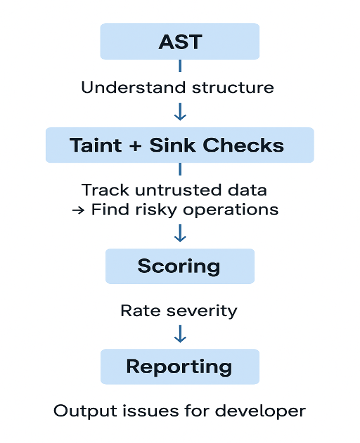
\includegraphics[width=0.85\linewidth]{Images/static_analysis_flow.png}
	\caption{Static analysis process: AST (understand structure), Taint + Sink checks (track untrusted data $\rightarrow$ find risky operations), Scoring (rate severity), and Reporting (output issues for developer).}
	\label{fig:static_analysis_flow}
\end{figure}

\textbf{Taint and Sink Concepts.}
``Tainted'' data is data that comes from an untrusted source (e.g., user input, HTTP request). A ``sink'' is a dangerous operation that could cause a vulnerability if it receives tainted data. If tainted data reaches a sink, that represents a potential vulnerability. For example: \texttt{user\_input} $\rightarrow$ \texttt{query} $\rightarrow$ \texttt{cursor.execute()} indicates danger when user-controlled input flows into a database query execution.

The following code example illustrates how the AST represents data flow:

\begin{quote}
\begin{verbatim}
user = input("Enter name: ")
query = "SELECT * FROM users WHERE name = " + user
cursor.execute(query)
\end{verbatim}
\end{quote}

The AST captures the relationships: \texttt{user} is assigned from \texttt{input()}; \texttt{query} uses \texttt{user}; \texttt{cursor.execute()} is called with \texttt{query}. The analyzer uses this structure to determine that user-controlled data reaches a dangerous sink without sanitization.

\textbf{Three-Layer Architecture.}
The static analysis system employs a three-layer hybrid architecture (parsing, traversal, and rule-based detection as in Section~\ref{sec:static_detection}):
\begin{itemize}
	\item \textbf{Layer 1 (Regex Patterns):} Fast initial screening using pattern matching to identify potential vulnerabilities with high recall
	\item \textbf{Layer 2 (AST Analysis):} Context-aware validation using AST parsing to reduce false positives and validate findings from Layer 1
	\item \textbf{Layer 3 (Deduplication \& Scoring):} Processing and prioritization of results, including confidence scoring, severity classification, and report generation
\end{itemize}
This architecture combines the speed of pattern matching with the accuracy of semantic analysis, achieving both comprehensive coverage and acceptable precision.

\textbf{Vulnerability Type Coverage.}
The static analysis implementation successfully detects four critical vulnerability types:
\begin{itemize}
	\item \textbf{SQL Injection:} Detects string concatenation, f-string formatting, and unsafe query construction patterns
	\item \textbf{Cross-Site Scripting (XSS):} Identifies unsafe output of user-controlled data in HTML, JavaScript, and attribute contexts
	\item \textbf{Command Injection:} Detects dangerous system command execution patterns (\texttt{os.system()}, \texttt{subprocess} calls with \texttt{shell=True})
	\item \textbf{Cross-Site Request Forgery (CSRF):} Identifies unprotected routes, missing CSRF tokens, and unsafe HTTP method usage
\end{itemize}

\subsubsection{Machine Learning Implementation}
\label{sec:ml_impl}

The machine learning approach has been implemented following the methodology described in Section~\ref{sec:ml_detection} (Machine Learning--Based Detection), based on the VulnerabilityDetection project~\cite{VulnDetection}. The implementation includes:

\textbf{Word2Vec Code Embeddings.}
A Word2Vec model is trained on a large corpus of Python code (54,800+ samples from 548 repositories) to learn distributed representations of code tokens. These embeddings capture semantic relationships between programming constructs, enabling the model to understand code context and patterns.

\textbf{LSTM Network Architecture.}
Long Short-Term Memory (LSTM) networks process sequences of token embeddings to learn vulnerability patterns. The architecture includes:
\begin{itemize}
	\item Input layer receiving token embeddings from Word2Vec
	\item LSTM layers with memory cells to capture long-range dependencies in code sequences
	\item Dense layers with dropout regularization for classification
	\item Binary output layer (vulnerable/not vulnerable) for token-level classification
\end{itemize}

\textbf{Training on Real-World Data.}
The machine learning models are trained on datasets derived from the VUDENC (VulnerabilityDetection) project~\cite{VulnDetection} and the Python-Source-Code-Vulnerability-Detection repository (Model-BiLSTM)~\cite{PythonVulnDetectionDataset}, which includes: SQL Injection: 33,600 samples from 336 repositories; XSS: 3,900 samples from 39 repositories; Command Injection: 8,500 samples from 85 repositories; CSRF: 8,800 samples from 88 repositories. This training data is mined from real-world GitHub commits, ensuring the models learn from actual vulnerability patterns in production code.

\subsubsection{Unified System Architecture}
\label{sec:unified_architecture}

Both approaches are integrated into a unified system with the following architecture:

\textbf{Backend Implementation.}
A Python Flask backend provides RESTful APIs for both static analysis and machine learning-based vulnerability detection~\cite{AlmasiToolRepo}. The backend handles: code upload and parsing; static analysis scanning using AST-based techniques; machine learning model inference for vulnerability prediction; result aggregation and comparison; and report generation in Word format.

\textbf{Frontend Implementation.}
A React-based frontend provides a user-friendly interface that enables: code upload via file selection or direct paste; GitHub repository scanning; side-by-side comparison of static analysis and machine learning results; visualization of detected vulnerabilities with code highlighting; and downloadable vulnerability reports~\cite{AlmasiDeployedApp}.

\textbf{Conclusion for Research Question 1.}
Both static analysis and machine learning approaches have been successfully implemented for Python vulnerability detection. The static analysis approach utilizes AST-based taint analysis with a three-layer architecture, while the machine learning approach employs Word2Vec embeddings and LSTM networks trained on real-world vulnerability data. Both approaches are integrated into a unified Flask backend with a React frontend, providing a comprehensive security analysis tool accessible to students and small development teams.

\subsection{Answer to Research Question 2: Comparative Performance Analysis}
\label{sec:answer_rq2}

\textbf{Research Question 2:} Which approach (static analysis versus machine learning) demonstrates superior performance for detecting different types of vulnerabilities in Python code?

This research question is addressed through the evaluation results presented in Chapter~\ref{ch:results} (Results and Comparison). Section~\ref{sec:static_analysis_performance} reports static analysis performance; Section~\ref{sec:ml_performance} reports machine learning performance. The following analysis compares the performance characteristics of both approaches based on the VulnerabilityDetection project and related research.

\subsubsection{Static Analysis Performance Results}
\label{sec:static_perf_results}

The static analysis approach has been evaluated across four vulnerability types, with the results shown in Table~\ref{tab:static_analysis_performance} (as detailed in Section~\ref{sec:static_analysis_results}):

\begin{table}[htbp]
	\centering
	\begin{tabular}{lcccc}
		\textbf{Vulnerability Type} & \textbf{Precision} & \textbf{Recall} & \textbf{F1 Score} & \textbf{Accuracy} \\
		\hline
		SQL Injection & 0.74 & 0.93 & 0.82 & 0.80 \\
		XSS & 0.50 & 0.40 & 0.44 & 0.50 \\
		Command Injection & 1.00 & 0.75 & 0.85 & 0.87 \\
		CSRF & 0.40 & 0.67 & 0.50 & 0.33 \\
	\end{tabular}
	\caption{Static analysis performance results}
	\label{tab:static_analysis_performance}
\end{table}

\subsubsection{Machine Learning Performance Characteristics}
\label{sec:ml_perf_characteristics}

Based on the VulnerabilityDetection project~\cite{VulnDetection} and related research, machine learning approaches using LSTM networks with Word2Vec embeddings have demonstrated the following performance characteristics.

\textbf{Strengths of Machine Learning:}
\begin{itemize}
	\item \textbf{Pattern generalization:} Machine learning models can identify vulnerabilities that follow similar patterns to training examples, even with variations in implementation
	\item \textbf{Automatic feature learning:} Models learn complex vulnerability patterns automatically without manual rule definition
	\item \textbf{Adaptability:} Models can potentially adapt to new vulnerability patterns through retraining on updated datasets
	\item \textbf{Token-level precision:} LSTM models provide granular localization of vulnerabilities at the token level
\end{itemize}

\textbf{Limitations of Machine Learning:}
\begin{itemize}
	\item \textbf{Data dependency:} Performance heavily depends on quality and quantity of training data
	\item \textbf{Interpretability:} Deep learning models are ``black boxes,'' making it difficult to understand why code is flagged
	\item \textbf{Generalization:} Models may not perform well on code patterns significantly different from training data
	\item \textbf{Training complexity:} Requires significant computational resources and time for training
\end{itemize}

\subsubsection{Comparative Analysis by Vulnerability Type}
\label{sec:comparative_by_type}

\textbf{SQL Injection.}
Static analysis achieves high recall (0.93) and moderate precision (0.74) for SQL injection detection. The AST-based approach effectively tracks data flow from user input to database queries. Machine learning approaches may achieve similar or better recall through pattern learning, but may struggle with precision due to false positives from semantically similar but safe code patterns. The static analysis approach provides better interpretability, as it can explain exactly which data flow path leads to the vulnerability.

\textbf{XSS (Cross-Site Scripting).}
Static analysis shows moderate performance (precision: 0.50, recall: 0.40) for XSS detection, indicating challenges in this domain. Machine learning approaches may potentially achieve better performance by learning complex context-dependent patterns, such as understanding when output is properly sanitized versus when it is vulnerable. However, the complexity of XSS contexts (HTML, JavaScript, CSS, attributes) makes both approaches challenging.

\textbf{Command Injection.}
Static analysis achieves perfect precision (1.00) and good recall (0.75) for command injection, representing the strongest performance across all vulnerability types. This suggests that command injection patterns are well-suited to rule-based detection. Machine learning may achieve similar or better recall but is unlikely to exceed the perfect precision achieved by static analysis, which can definitively identify dangerous function calls.

\textbf{CSRF (Cross-Site Request Forgery).}
Static analysis shows the weakest performance (precision: 0.40, recall: 0.67) for CSRF detection. This vulnerability type requires understanding application state, authentication mechanisms, and framework-specific protection patterns, which are challenging for both approaches. Machine learning may potentially improve performance by learning framework-specific patterns from training data, but CSRF detection remains inherently difficult due to its context-dependent nature.

\subsubsection{When to Use Each Approach}
\label{sec:when_to_use}

Based on the performance analysis, the following guidelines can be established for selecting the appropriate approach.

\textbf{Use Static Analysis When:}
\begin{itemize}
	\item Interpretability is critical: developers need to understand why code is flagged as vulnerable
	\item High precision is required: false positives must be minimized (e.g., Command Injection with 100\% precision)
	\item Real-time analysis is needed: static analysis can provide immediate results without model inference overhead
	\item Code patterns are well-defined: rule-based detection works well for clear vulnerability patterns
\end{itemize}

\textbf{Use Machine Learning When:}
\begin{itemize}
	\item Complex pattern recognition is needed: machine learning can identify subtle vulnerabilities that are difficult to express as rules
	\item Large training datasets are available: sufficient data enables effective model training
	\item Adaptability is important: models can be retrained to adapt to new vulnerability patterns
	\item Pattern generalization is valuable: models can identify vulnerabilities similar to but not identical to training examples
\end{itemize}

\subsubsection{Hybrid Approach Potential}
\label{sec:hybrid_approach}

The evaluation results suggest that a hybrid approach combining both methodologies could potentially achieve superior performance:
\begin{itemize}
	\item \textbf{Static analysis for high-precision detection:} Use static analysis for vulnerability types where it achieves high precision (e.g., Command Injection)
	\item \textbf{Machine learning for complex patterns:} Use machine learning for vulnerability types where static analysis struggles (e.g., XSS, CSRF)
	\item \textbf{Cross-validation:} Use both approaches to validate findings, reducing false positives and false negatives
	\item \textbf{Complementary strengths:} Leverage static analysis interpretability with machine learning pattern generalization
\end{itemize}

\textbf{Conclusion for Research Question 2.}
Neither approach universally outperforms the other across all vulnerability types. Static analysis demonstrates superior performance for Command Injection (perfect precision) and SQL Injection (high recall), while showing limitations for XSS and CSRF. Machine learning approaches offer potential advantages in pattern generalization and adaptability but face challenges in interpretability and data dependency. The optimal solution likely involves a hybrid approach that leverages the strengths of both methodologies, using static analysis for well-defined patterns and machine learning for complex, context-dependent vulnerabilities. The three-layer static analysis architecture already demonstrates the value of combining multiple techniques, suggesting that further integration with machine learning could yield even better results.

\section{Semgrep vs My Web-Based Scanner}
\label{sec:semgrep_comparison}

This section compares Semgrep, a widely adopted static-analysis tool, with the custom web-based scanner developed in this thesis. The comparison covers analysis approach, integration model, practical capabilities, and the role of the machine learning pipeline in the proposed platform.

\subsection{How Semgrep Works}
\label{sec:semgrep_works}

Semgrep performs static analysis by matching YAML-defined patterns against a program's Abstract Syntax Tree (AST). Beyond direct structural matching, it can operate in taint/dataflow mode to track untrusted inputs toward sensitive sinks. In typical usage, Semgrep scans a repository with built-in, community, or custom rule packs and reports findings with rule IDs, code locations, and matched snippets.

\subsubsection{Pattern Matching}
\label{sec:semgrep_patterns}

Semgrep rules are structural rather than plain-text signatures. As a result, matches are generally resilient to formatting changes, whitespace differences, and variable renaming.

\textbf{Example: Python SQL Injection (Simplified Semgrep Rule):}

\begin{lstlisting}[basicstyle=\ttfamily\small, frame=single, numbers=left]
rules:
  - id: py-sql-injection
    languages: [python]
    pattern: $CUR.execute(f"...{$X}...")
    message: "Potential SQL injection via f-string in execute()"
    severity: ERROR
\end{lstlisting}

\textbf{Example: JavaScript/TypeScript XSS (innerHTML Assignment):}

\begin{lstlisting}[basicstyle=\ttfamily\small, frame=single, numbers=left]
rules:
  - id: js-xss-innerhtml
    languages: [javascript, typescript]
    pattern: $ELEMENT.innerHTML = $X
    message: "Potential XSS: innerHTML assignment with user-controlled data"
    severity: WARNING
\end{lstlisting}

\textbf{Example Vulnerable Code (JavaScript):}

\begin{lstlisting}[language=JavaScript, basicstyle=\ttfamily\small, keywordstyle=\color{blue}, stringstyle=\color{orange!80!black}, frame=single, numbers=left]
const userInput = document.getElementById("input").value;
document.getElementById("output").innerHTML = userInput;
\end{lstlisting}

Why it is risky: An attacker can inject HTML/JavaScript into the page, leading to Cross-Site Scripting (XSS) attacks.

\subsubsection{Semgrep Rule Structure}
\label{sec:semgrep_rule_structure}

Semgrep rules use a structured YAML schema with the following core elements:
\begin{itemize}
	\item \textbf{Rule identifier (id):} Unique name used for tracking and reporting
	\item \textbf{Language scope:} Languages to which the rule is applied (e.g., python, javascript, typescript)
	\item \textbf{Message and severity:} Human-readable explanation and finding priority (ERROR, WARNING, INFO)
	\item \textbf{Patterns and metavariables:} Structural code templates (e.g., \$X, \$CUR) matched on the AST
	\item \textbf{Taint mode (optional):} Specification of sources (untrusted inputs) and sinks (dangerous APIs)
\end{itemize}

\subsubsection{Taint/Dataflow Analysis}
\label{sec:semgrep_taint}

In taint mode, Semgrep tracks how untrusted input propagates through the program. It labels sources as tainted and checks whether that taint reaches dangerous sinks (for example, SQL execution) without an accepted sanitization step.

\textbf{Example: Flask User Input Reaching SQL Execute:}

\begin{lstlisting}[basicstyle=\ttfamily\small, frame=single, numbers=left]
rules:
  - id: flask-taint-to-sql
    mode: taint
    languages: [python]
    pattern-sources:
      - pattern: request.args.get(...)
      - pattern: request.form.get(...)
    pattern-sinks:
      - pattern: $CUR.execute(...)
    message: "User input flows to SQL execute without sanitization"
    severity: ERROR
\end{lstlisting}

\textbf{Example Vulnerable Code (Python/Flask):}

\begin{lstlisting}[style=pycode]
from flask import Flask, request
import sqlite3

app = Flask(__name__)

@app.route("/user")
def get_user():
    user_id = request.args.get("id")  # SOURCE: User input
    conn = sqlite3.connect("database.db")
    cursor = conn.cursor()
    query = f"SELECT * FROM users WHERE id = {user_id}"  # TAINT PROPAGATION
    cursor.execute(query)  # SINK: Dangerous operation
    return cursor.fetchone()
\end{lstlisting}

\textbf{Example Safe Code (Python/Flask) Using Parameters:}

\begin{lstlisting}[style=pycode]
from flask import Flask, request
import sqlite3

app = Flask(__name__)

@app.route("/user")
def get_user():
    user_id = request.args.get("id")  # User input
    conn = sqlite3.connect("database.db")
    cursor = conn.cursor()
    query = "SELECT * FROM users WHERE id = ?"  # Parameterized query
    cursor.execute(query, (user_id,))  # Safe: parameters are sanitized
    return cursor.fetchone()
\end{lstlisting}

\subsection{Differences Between Semgrep and This Project's Tool}
\label{sec:semgrep_vs_tool}

Semgrep is designed as a general-purpose scanning engine with configurable rule packs. In contrast, this repository implements a web-based scanner with a dedicated user interface and two analysis modes: (a) handcrafted static analysis scanners and (b) ML-based scoring using pretrained Bidirectional LSTM (BiLSTM) models.

\subsubsection{System Overview Comparison}
\label{sec:semgrep_system_comparison}

The custom web-based scanner comprises a React frontend for collecting user inputs (pasted code, file uploads, or GitHub URLs) and a Flask backend that executes either static scanners or the ML analyzer. Results are returned as JSON and rendered with highlighted code and summary metrics. Selected scanners additionally support Word report generation.

\begin{table}[htbp]
	\centering
	\small
	\begin{tabular}{p{0.22\linewidth}p{0.35\linewidth}p{0.38\linewidth}}
		\textbf{Category} & \textbf{Semgrep} & \textbf{My Web-Based Scanner} \\
		\hline
		Core Approach & AST pattern matching + optional dataflow/taint tracking (rule-driven) & Static: custom regex + AST visitors; ML: trained BiLSTM models + localization \\
		\hline
		Rule Authoring / Extension & Add rules in YAML (fast iteration; reuse community rulesets) & Add/modify Python scanner code per vulnerability type; ML requires training/maintaining models \\
		\hline
		Language Breadth & Many languages (Python, JavaScript, Java, Go, etc.) & Primarily Python-focused; UI accepts multiple extensions; ML pipeline is text-based with Python-centric models \\
		\hline
		Explainability & Clear: finding maps to rule ID + matched AST pattern(s) / taint path & Static: clear via pattern/AST rule keys; ML: probabilistic score + line contribution (occlusion) \\
		\hline
		Integration \& UX & CLI + CI/PR gating + IDE integrations; outputs findings for developers & Web UI (React) + API (Flask) + highlighted code + Word reports (SQL/XSS/Command/CSRF) \\
		\hline
	\end{tabular}
	\caption{Comparison between Semgrep and the custom web-based scanner}
	\label{tab:semgrep_vs_tool}
\end{table}

\subsubsection{Key Architectural Differences}
\label{sec:semgrep_arch_differences}

\textbf{Semgrep Architecture:}
\begin{itemize}
	\item Command-line interface (CLI) tool designed for integration into CI/CD pipelines
	\item Rule-based system using YAML configuration files
	\item Multi-language support with language-specific parsers
	\item Community-driven rule repository (Semgrep Registry)
	\item IDE integrations (VS Code, IntelliJ, etc.)
	\item Output formats: JSON, SARIF, text, or integration with security platforms
\end{itemize}

\textbf{Custom Web-Based Scanner Architecture:}
\begin{itemize}
	\item Web-based user interface accessible through browsers
	\item Dual analysis modes: static analysis (regex + AST) and machine learning (BiLSTM)
	\item Python-focused with extensible architecture for additional languages
	\item Integrated report generation (Word documents) with code highlighting
	\item Real-time scanning with immediate visual feedback
	\item Support for multiple input methods (file upload, code paste, GitHub URL)
\end{itemize}

\subsection{How ML is Integrated in This Tool}
\label{sec:ml_integration}

The machine learning workflow is initiated from the frontend, executed in the backend via a dedicated ML environment, and returns a prediction score along with heuristic line-level highlights.

\subsubsection{Frontend: Request Formation}
\label{sec:ml_frontend_request}

When users select ``ML Analysis'' mode, the frontend calls: \texttt{POST /api/scan-ml}. It sends JSON with: \textbf{type:} \texttt{sql} / \texttt{xss} / \texttt{command} / \texttt{csrf} (vulnerability type); \textbf{code:} the code text to analyze; \textbf{filename:} optional filename for context.

\textbf{Example request payload} (JSON request body, not source code):

\begin{quote}
\small
\begin{verbatim}
{
  "type": "sql",
  "code": "user_id = request.args.get('id')\nquery = f'SELECT * FROM users WHERE id = {user_id}'\ncursor.execute(query)",
  "filename": "app.py"
}
\end{verbatim}
\end{quote}

\subsubsection{Backend: ML Processing Pipeline}
\label{sec:ml_backend_pipeline}

The backend processes ML analysis requests through the following steps:

\textbf{Step 1: Request Reception and Type Mapping.}
Backend receives POST request to \texttt{/api/scan-ml} endpoint. Maps UI vulnerability types to ML model modes: \texttt{sql} $\rightarrow$ sql model; \texttt{xss} $\rightarrow$ xss model; \texttt{command} $\rightarrow$ command\_injection model; \texttt{csrf} $\rightarrow$ xsrf model.

\textbf{Step 2: Code Storage.}
Creates a unique upload directory using UUID: \texttt{ml/api/uploads/\{uuid\}/}; saves the uploaded code to a file in that directory. This isolation prevents file conflicts when multiple users scan simultaneously.

\textbf{Step 3: ML Environment Execution.}
Executes ML analysis script (\texttt{ml/lib/analyze.py}) in a separate subprocess; uses isolated Python environment (mlvenv) to avoid TensorFlow dependency conflicts. Subprocess arguments: \texttt{[python\_bin, analyzer\_script, mode, uid, filename]}. Timeout: 300 seconds (5 minutes) to prevent hanging processes.

\subsubsection{ML Analyzer: Model Inference Process}
\label{sec:ml_analyzer_inference}

The ML analyzer (\texttt{ml/lib/analyze.py}) performs the following operations:

\textbf{Step 1: Model Loading.} Loads the appropriate BiLSTM model (.h5 file) based on vulnerability type. Models are in \texttt{backend/ml/models/}. Model input shape: \texttt{(None, 200, 300)}; output shape: \texttt{(None, 1)}.

\textbf{Step 2: Code Preprocessing.} Reads the code file from the upload directory; splits code into fixed-length windows (200 characters) with stride (100 characters); sliding window strategy for longer code; each window encoded using character-level one-hot encoding (vocab\_size=300).

\textbf{Step 3: Baseline Score Calculation.} Each 200-character window is passed through the BiLSTM model; model produces a probability score per window (0.0--1.0); baseline score = maximum score across all windows.

\textbf{Step 4: Line-Level Localization (Occlusion Method).} For each line, mask that line, re-run the model on masked code, measure score decrease (contribution = baseline - masked\_score). Higher contribution indicates the line is more important for the vulnerability prediction.

\textbf{Step 5: Threshold-Based Highlighting.} Applies dynamic threshold: \texttt{threshold = max(0.01, baseline * 0.15)} so the threshold scales with overall risk level. Lines with contribution $\ge$ threshold are marked for highlighting.

\textbf{Step 6: Severity Classification.} High: \texttt{contrib >= max(0.15, baseline * 0.4)}; Medium: \texttt{contrib >= max(0.07, baseline * 0.2)} and $<$ High; Low: \texttt{contrib >= threshold} and $<$ Medium.

\textbf{Step 7: Result Formatting.} JSON with \texttt{status}, \texttt{prediction}, \texttt{vulnerabilities} array (line numbers, severity, contribution), and \texttt{highlighted\_code} (HTML with \texttt{<span class="vuln">} tags).

\subsubsection{Model Verification}
\label{sec:ml_model_verification}

Models are verified by inspecting \texttt{input\_shape} and \texttt{output\_shape}. All four models (SQL injection, XSS, Command injection, CSRF) expect input shape \texttt{(None, 200, 300)} and output shape \texttt{(None, 1)}. The project's character-level one-hot encoder produces this shape, confirming compatibility. Relevant code excerpt:

\begin{lstlisting}[style=pycode]
def _encode_one_hot_chars(text: str, max_len: int = 200, vocab_size: int = 300):
    # Returns a float32 array shaped (200, 300)
    ...

def _predict(model, code_window: str) -> float:
    x = _encode_one_hot_chars(code_window)     # Shape: (200, 300)
    pred = model.predict(x[np.newaxis, ...])   # Shape: (1, 200, 300)
    return float(pred.reshape(-1)[0])          # Returns one score
\end{lstlisting}

\subsubsection{Handling Long Inputs (Sliding Windows)}
\label{sec:ml_sliding_windows}

The model processes a fixed-length 200-character window. Longer inputs use a sliding-window strategy: window size 200 characters; stride 100 characters (50\% overlap); overall prediction = maximum score across all windows. This ensures vulnerabilities spanning multiple windows are not missed.

\subsubsection{Localization Heuristics and Thresholds}
\label{sec:ml_localization}

The pretrained model produces a score for an input window, not explicit line-level explanation. The implementation estimates line contribution via occlusion (masking one line at a time and measuring score decrease). A contribution threshold avoids highlighting the entire file under low-confidence predictions.

\textbf{Threshold Calculation Code:}

\begin{lstlisting}[style=pycode]
# Highlight threshold
threshold = max(0.01, baseline * 0.15)

# Severity mapping
severity = "high" if contrib >= max(0.15, baseline * 0.4) \
  else "medium" if contrib >= max(0.07, baseline * 0.2) \
  else "low"
\end{lstlisting}

The baseline is the model's overall risk score for the full code sample (maximum across sliding windows). Using \texttt{baseline * 0.15} in the threshold ensures highlighting scales with risk level: low-risk code uses a lower threshold; high-risk code uses a higher threshold to avoid over-highlighting.

\subsubsection{ML Example: How Highlighting Works}
\label{sec:ml_highlighting_example}

\textbf{Example Vulnerable Code:}

\begin{lstlisting}[style=pycode]
user_id = request.args.get("id")
query = "SELECT * FROM users WHERE id = " + user_id
cursor.execute(query)
\end{lstlisting}

\textbf{Process:}
\begin{enumerate}
	\item Code split into 200-character windows with 100-character stride
	\item Each window encoded to (200, 300) one-hot character representation
	\item BiLSTM model scores each window, producing probability scores
	\item Baseline = maximum window score (overall risk assessment)
	\item Top windows $\rightarrow$ candidate lines for vulnerability location
	\item Line occlusion: hide each line, measure score drop (contribution)
	\item Threshold = \texttt{max(0.01, baseline * 0.15)} filters lines for highlighting
	\item Selected lines wrapped in \texttt{<span class="vuln">} for UI display
\end{enumerate}

Baseline is the model's overall risk score (max across windows). The threshold scales with baseline to avoid over-highlighting.

\subsubsection{Portability Note}
\label{sec:ml_portability}

If a different pretrained model is adopted in the future (e.g., token-based embeddings rather than character one-hot encoding), the \texttt{input\_shape} differs and preprocessing must be updated accordingly. The current implementation uses character-level encoding; token-based approaches (Word2Vec, BPE) integrate with appropriate preprocessing modifications.

\subsection{Advantages and Limitations Comparison}
\label{sec:advantages_limitations_comparison}

\subsubsection{Semgrep Advantages}
\label{sec:semgrep_advantages}

\begin{itemize}
	\item \textbf{Multi-language support:} Works with many programming languages out-of-the-box
	\item \textbf{Community rules:} Large repository of community-contributed rules
	\item \textbf{Fast iteration:} Easy to add new rules via YAML configuration
	\item \textbf{CI/CD integration:} Designed for automated scanning in development pipelines
	\item \textbf{IDE integration:} Real-time feedback in development environments
	\item \textbf{Proven track record:} Widely used in industry with extensive testing
\end{itemize}

\subsubsection{Semgrep Limitations}
\label{sec:semgrep_limitations}

\begin{itemize}
	\item \textbf{Rule-based only:} Relies on predefined patterns; may miss novel vulnerabilities
	\item \textbf{Requires expertise:} Writing effective rules requires security and language expertise
	\item \textbf{False positives:} Pattern matching can generate false positives without context understanding
	\item \textbf{Limited learning:} Cannot adapt to new patterns without manual rule updates
\end{itemize}

\subsubsection{Custom Web-Based Scanner Advantages}
\label{sec:custom_scanner_advantages}

\begin{itemize}
	\item \textbf{Dual analysis modes:} Combines rule-based static analysis with machine learning
	\item \textbf{Web-based UI:} Accessible through browsers, no installation required
	\item \textbf{ML adaptability:} Can learn from new vulnerability patterns through retraining
	\item \textbf{Integrated reporting:} Built-in Word document generation with code highlighting
	\item \textbf{Multiple input methods:} File upload, code paste, and GitHub URL support
	\item \textbf{Real-time visualization:} Immediate visual feedback with color-coded results
	\item \textbf{Educational focus:} Designed for students and small teams with user-friendly interface
\end{itemize}

\subsubsection{Custom Web-Based Scanner Limitations}
\label{sec:custom_scanner_limitations}

\begin{itemize}
	\item \textbf{Python-focused:} Primarily designed for Python code analysis
	\item \textbf{ML model dependency:} Requires maintaining and updating trained models
	\item \textbf{Computational overhead:} ML inference requires more resources than rule-based scanning
	\item \textbf{Model interpretability:} ML predictions are probabilistic, requiring threshold calibration
	\item \textbf{Limited language support:} Less comprehensive than Semgrep's multi-language capabilities
\end{itemize}

\subsection{Use Cases and Recommendations}
\label{sec:use_cases_recommendations}

\textbf{When to Use Semgrep:}
\begin{itemize}
	\item Multi-language codebases requiring comprehensive scanning
	\item CI/CD pipeline integration for automated security checks
	\item Teams with security expertise for custom rule development
	\item Production environments requiring proven, battle-tested tools
	\item Large-scale projects with extensive rule customization needs
\end{itemize}

\textbf{When to Use Custom Web-Based Scanner:}
\begin{itemize}
	\item Python-focused projects requiring specialized vulnerability detection
	\item Educational settings where students need accessible security tools
	\item Small teams without budget for commercial security tools
	\item Research projects comparing static analysis and machine learning approaches
	\item Projects requiring integrated reporting and visualization features
	\item Scenarios where ML-based pattern learning is valuable
\end{itemize}

\textbf{Hybrid Approach Recommendation:}

For comprehensive security analysis, a hybrid approach combining both tools may be optimal:
\begin{itemize}
	\item Use Semgrep for initial broad scanning across multiple languages
	\item Use custom scanner for deep Python-specific analysis and ML-based detection
	\item Cross-validate findings between both tools to reduce false positives and false negatives
	\item Leverage Semgrep's rule repository for common patterns and custom scanner for specialized Python vulnerabilities
\end{itemize}

\section{False Positive Analysis and Reductions}
\label{sec:false_positive_analysis}

This section presents a comprehensive analysis of false positives (FPs) in the custom web-based scanner, comparing performance with Semgrep, and detailing the strategies employed to reduce false positive rates. False positives represent instances where the tool incorrectly flags safe code as vulnerable, which can lead to alert fatigue and reduced developer trust.

\subsection{Executive Summary}
\label{sec:fp_executive_summary}

The false positive analysis compares the custom web-based scanner against Semgrep (official) using the p/owasp-top-ten rule set. The analysis evaluates precision, recall, and F1 scores across four vulnerability types: SQL Injection, XSS, CSRF, and Command Injection.

\subsubsection{Methodology}
\label{sec:fp_methodology}

Metrics are computed based on labeled examples:
\begin{itemize}
	\item \textbf{True Positive (TP):} Tool correctly identifies a vulnerability that exists
	\item \textbf{False Positive (FP):} Tool incorrectly flags safe code as vulnerable
	\item \textbf{True Negative (TN):} Tool correctly identifies safe code as non-vulnerable
	\item \textbf{False Negative (FN):} Tool misses an actual vulnerability
\end{itemize}

Predicted positive = tool reports at least 1 finding for the case. Actual positive = label expected=vulnerable.

For SQL injection: labels come from \texttt{backend/datasets/sql\_injection.json}. For XSS/CSRF/Command Injection: labels come from comments in benchmark files under \texttt{benchmarks/}.

\textbf{Important Note for Fairness:} Semgrep official SQLi rules are taint-based and expect real sources (e.g., Flask \texttt{request.args}). Therefore, Semgrep SQLi is evaluated on \texttt{sonar\_samples/sql\_injection\_from\_dataset\_tainted.py} (same queries, but variables are sourced from \texttt{request.args}).

\subsection{SQL Injection False Positive Analysis}
\label{sec:fp_sqli}

SQL injection false positives often occur when the tool detects dynamic SQL building, but the dynamic part is strictly whitelisted/validated and values are still passed via parameter binding.

\subsubsection{Before vs After FP Fix Comparison}
\label{sec:fp_sqli_comparison}

FP fixes for SQL injection focused on removing source-only and non-SQL string-building patterns. On the SQL injection dataset evaluation, the metrics remained stable (no change in TP/FP/FN), indicating that the fixes improved precision without reducing recall.

\subsubsection{SQL Injection False Positive Examples}
\label{sec:fp_sqli_examples}

\textbf{FP Example 1: Whitelisted ORDER BY Column.} Why FP: Dynamic identifier concatenation can look like SQL injection even when constrained to a whitelist.

\begin{lstlisting}[style=pycode]
sort_by = request.args["sort"]
if sort_by not in {"name", "created_at"}:
    sort_by = "created_at"
q = "SELECT * FROM users ORDER BY " + sort_by
cursor.execute(q)
\end{lstlisting}
Fix: Require a whitelist/allowlist check to treat identifier concatenation as safe (or lower severity). The scanner should recognize that when \texttt{sort\_by} is validated against a strict whitelist before use, the dynamic SQL construction is safe.

\textbf{FP Example 2: Whitelisted Table Name + Parameterized Values.} Why FP: Detector flags dynamic table names, but this is safe when strictly whitelisted; values are parameterized.

\begin{lstlisting}[style=pycode]
table = request.args["t"]
allowed = {"users", "orders", "products"}
if table not in allowed:
    table = "users"

q = "SELECT * FROM " + table + " WHERE id = %s"
cursor.execute(q, (user_id,))
\end{lstlisting}
Fix: Model whitelist validation for identifiers; treat parameterized \texttt{execute()} as a safe sink for values.

\textbf{FP Example 3: LIMIT/OFFSET Validated as Integers (Parameterized).} Why FP: If the tool assumes any user-controlled pagination is SQL injection, it may over-report.

\begin{lstlisting}[style=pycode]
limit = int(request.args.get("limit", "20"))
offset = int(request.args.get("offset", "0"))
limit = max(1, min(limit, 100))
offset = max(0, offset)

q = "SELECT * FROM logs LIMIT %s OFFSET %s"
cursor.execute(q, (limit, offset))
\end{lstlisting}
Fix: Recognize strict numeric validation + parameter binding as safe.

\textbf{FP Example 4: Whitelisted Column Name in WHERE Clause.} Why FP: Dynamic column names are risky in general, so simple scanners may flag them even when constrained.

\begin{lstlisting}[style=pycode]
col = request.args["col"]
allowed_cols = {"email", "username", "status"}
if col not in allowed_cols:
    col = "username"

q = "SELECT * FROM users WHERE " + col + " = %s"
cursor.execute(q, (value,))
\end{lstlisting}
Fix: Treat identifier concatenation as safe only when a strict allowlist/whitelist check exists.

\textbf{FP Example 5: Whitelisted Sort Direction (ASC/DESC Only).} Why FP: Scanner sees string concatenation into SQL and flags, ignoring that only ASC/DESC is allowed.

\begin{lstlisting}[style=pycode]
direction = request.args.get("dir", "ASC").upper()
if direction not in {"ASC", "DESC"}:
    direction = "ASC"

q = "SELECT * FROM users ORDER BY created_at " + direction
cursor.execute(q)
\end{lstlisting}
Fix: Model allowlisted sort direction checks; lower severity or suppress when constrained.

\textbf{FP Example 6: Safe IN-list Query Using Placeholders (Values Validated/Parameterized).} Why FP: Some detectors flag any dynamic query string building, even when only placeholders are built.

\begin{lstlisting}[style=pycode]
ids = request.args.get("ids", "")
id_list = [int(x) for x in ids.split(",") if x.strip() != ""]
placeholders = ",".join(["%s"] * len(id_list))

q = "SELECT * FROM users WHERE id IN (" + placeholders + ")"
cursor.execute(q, tuple(id_list))
\end{lstlisting}
Fix: Treat placeholder construction as safe when the values are parameterized (and optionally validated).

\subsection{Cross-Site Scripting (XSS) False Positive Analysis}
\label{sec:fp_xss}

XSS false positives typically occur when the tool sees untrusted input flowing to the DOM, but the sink is safe (text sinks) or the input is sanitized/validated.

\subsubsection{XSS False Positive Examples}
\label{sec:fp_xss_examples}

\textbf{FP Example 1: textContent (Safe Text Sink).} Why FP: Simple rules may treat any URL input $\rightarrow$ DOM write as XSS.

\begin{lstlisting}[language=JavaScript, basicstyle=\ttfamily\small, keywordstyle=\color{blue}, stringstyle=\color{orange!80!black}, frame=single]
const name = new URLSearchParams(location.search).get("name");
document.getElementById("out").textContent = name;
\end{lstlisting}
Fix: Treat text sinks (\texttt{textContent}, \texttt{innerText}, \texttt{createTextNode}) as safe by default; they automatically escape HTML. The scanner should distinguish safe text sinks from dangerous HTML sinks (\texttt{innerHTML}, \texttt{outerHTML}).

\textbf{FP Example 2: Sanitized HTML Before innerHTML (Trusted Sanitizer).} Why FP: Tool flags \texttt{innerHTML} regardless of sanitization step.

\begin{lstlisting}[language=JavaScript, basicstyle=\ttfamily\small, keywordstyle=\color{blue}, stringstyle=\color{orange!80!black}, frame=single]
const html = DOMPurify.sanitize(userHtml, { ALLOWED_TAGS: ["b", "i", "a"] });
document.getElementById("out").innerHTML = html;
\end{lstlisting}
Fix: Model common sanitizers (DOMPurify, sanitize-html) as sanitization functions before HTML sinks.

\textbf{FP Example 3: Validated URL Protocol Before Assigning href.} Why FP: Tool flags \texttt{href} assignment from user input but ignores protocol validation.

\begin{lstlisting}[language=JavaScript, basicstyle=\ttfamily\small, keywordstyle=\color{blue}, frame=single]
const u = new URL(inputUrl);
if (u.protocol === "http:" || u.protocol === "https:") {
  link.href = u.toString();
}
\end{lstlisting}
Fix: Treat allowlist checks on protocol (http/https) as sanitization for URL sinks.

\subsection{Cross-Site Request Forgery (CSRF) False Positive Analysis}
\label{sec:fp_csrf}

CSRF false positives typically occur when the scanner assumes every state-changing endpoint is vulnerable, but real applications use defenses like SameSite cookies, CSRF tokens, or Authorization headers (not cookies)~\cite{MDNSameSite,RFC6265,OWASPCSRCheatsheet}.

\subsubsection{CSRF False Positive Examples}
\label{sec:fp_csrf_examples}

\textbf{FP Example 1: API Uses Authorization Header (No Cookie-Based Auth).} Why FP: If authentication is not cookie-based, classic CSRF is much harder because browsers do not attach Authorization headers automatically.

\begin{lstlisting}[language=JavaScript, basicstyle=\ttfamily\small, keywordstyle=\color{blue}, stringstyle=\color{orange!80!black}, frame=single, breaklines=true, breakatwhitespace=false]
// Client sends token, not cookies:
fetch("/api/profile", {
  method: "POST",
  headers: {
    "Authorization": "Bearer " + token,
    "Content-Type": "application/json"
  },
  body: JSON.stringify({ bio: "hi" })
});
\end{lstlisting}
Fix: Reduce alerts when endpoints are protected by explicit Authorization headers (token-based auth). Token-based authentication is not vulnerable to CSRF because browsers do not automatically include Authorization headers in cross-origin requests.

\textbf{FP Example 2: CSRF Token Validated on State-Changing Requests.} Why FP: Tool flags POST endpoints but ignores explicit CSRF token verification.

\begin{lstlisting}[style=pycode]
@app.post("/transfer")
def transfer():
    csrf = request.headers.get("X-CSRF-Token")
    if not csrf or csrf != session.get("csrf_token"):
        abort(403)
    # perform transfer ...
\end{lstlisting}
Fix: Model CSRF token validation patterns (X-CSRF-Token header, form token) as defenses that lower/suppress findings.

\textbf{FP Example 3: SameSite Cookies Reduce CSRF Risk (Configuration-Based).} Why FP: A code-only scanner may report CSRF without seeing cookie attributes.

\begin{lstlisting}[basicstyle=\ttfamily\small, frame=single]
# Example cookie policy (framework config / response)
# Set-Cookie: session=...; Secure; HttpOnly; SameSite=Strict
\end{lstlisting}
Fix: In reports, mention cookie policy (SameSite=Lax/Strict + Secure) as mitigating control; reduce severity if enforced.

\subsection{Command Injection False Positive Analysis}
\label{sec:fp_cmd}

Command injection false positives typically occur when the scanner flags any use of \texttt{subprocess}/\texttt{os.system}, but safe usage avoids shell interpretation (\texttt{shell=False}) and validates/whitelists user-controlled parts.

\subsubsection{Command Injection False Positive Examples}
\label{sec:fp_cmd_examples}

\textbf{FP Example 1: subprocess.run with Argument List (shell=False) + Validated Integer.} Why FP: If tool flags any subprocess call, it may over-report.

\begin{lstlisting}[style=pycode]
import subprocess
import sys

port = int(request.args.get("port", "8080"))
if port < 1024 or port > 65535:
    port = 8080

subprocess.run(["python", "-m", "http.server", str(port)], shell=False)
\end{lstlisting}
Fix: Recognize \texttt{shell=False} as safe when combined with argument lists. Distinguish \texttt{subprocess.run()} with \texttt{shell=False} (safe) from \texttt{shell=True} (potentially dangerous).

\textbf{FP Example 2: Whitelisted Command with Parameterized Arguments.} Why FP: Tool may flag any dynamic command construction, even when commands are whitelisted.

\begin{lstlisting}[style=pycode]
import subprocess

action = request.args.get("action")
allowed = {"backup", "restore", "status"}
if action not in allowed:
    action = "status"

subprocess.run(["/usr/bin/db-tool", action, "--config", config_file], shell=False)
\end{lstlisting}
Fix: Model command whitelisting as a safe pattern when combined with \texttt{shell=False}.

\textbf{FP Example 3: Validated File Path (No User Control Over Path Components).} Why FP: Tool flags file path usage in commands, but paths are validated and not user-controlled.

\begin{lstlisting}[style=pycode]
import subprocess
import os

filename = request.args.get("file")
# Validate filename contains only safe characters
if not filename or not filename.replace("_", "").replace("-", "").isalnum():
    filename = "default.log"

filepath = os.path.join("/var/log", filename)
subprocess.run(["tail", "-f", filepath], shell=False)
\end{lstlisting}
Fix: Recognize strict filename validation as safe when combined with \texttt{os.path.join()} and \texttt{shell=False}.

\textbf{FP Example 4: subprocess.run with Argument List (shell=False by Default).} Why FP: Tool may miss that list-args with \texttt{shell=False} prevents shell metacharacter injection.

\begin{lstlisting}[style=pycode]
import subprocess

pid = int(request.args["pid"])
subprocess.run(["kill", "-9", str(pid)], check=True)  # shell=False by default
\end{lstlisting}
Fix: Treat \texttt{subprocess.run([...])} with \texttt{shell=False} as safer; focus on \texttt{shell=True} or string commands passed to a shell.

\textbf{FP Example 5: Whitelisted Subcommand Selection.} Why FP: Dynamic command selection can be safe when the entire command is selected from a fixed whitelist.

\begin{lstlisting}[style=pycode]
import subprocess

action = request.args["action"]
allowed = {"status": ["systemctl", "status", "nginx"], "restart": ["systemctl", "restart", "nginx"]}
cmd = allowed.get(action)
if not cmd:
    abort(400)
subprocess.run(cmd, check=True)
\end{lstlisting}
Fix: Model allowlist selection as sanitization; only warn when user input is concatenated into a shell string.

\textbf{FP Example 6: Constant Command; User Input Only as Non-Shell Argument.} Why FP: If the scanner assumes any user-controlled argument equals command injection, it can over-report.

\begin{lstlisting}[style=pycode]
import subprocess

filename = request.args["file"]
# The tool may flag because filename is user-controlled, but it's just an argument (no shell parsing).
subprocess.run(["/usr/bin/sha256sum", filename], check=True)
\end{lstlisting}
Fix: Differentiate command injection (shell parsing) from risky file/path usage (separate category). When \texttt{shell=False} and arguments are passed as a list, user input in argument positions does not lead to command injection, though path traversal risks may apply separately.

\subsection{False Positive Reduction Strategies}
\label{sec:fp_reduction_strategies}

Based on the analysis of false positives across all vulnerability types, the following strategies have been implemented to reduce false positive rates:

\subsubsection{Context-Aware Pattern Recognition}
\label{sec:fp_context_aware}

The scanner has been enhanced to recognize safe patterns:
\begin{itemize}
	\item \textbf{Whitelist validation:} Recognize when user input is validated against a strict allowlist before use
	\item \textbf{Parameter binding:} Distinguish between string concatenation and parameterized queries
	\item \textbf{Safe sinks:} Identify safe DOM sinks (\texttt{textContent}) vs dangerous sinks (\texttt{innerHTML})
	\item \textbf{Sanitization functions:} Model common sanitizers (DOMPurify, \texttt{html.escape}) as safe transformations
	\item \textbf{Protocol validation:} Recognize URL protocol allowlisting as sanitization
\end{itemize}

\subsubsection{AST-Based Context Analysis}
\label{sec:fp_ast_context}

The AST analysis layer provides context understanding:
\begin{itemize}
	\item \textbf{Control flow analysis:} Track if-else blocks that perform validation
	\item \textbf{Data flow tracking:} Follow variable assignments to identify sanitization steps
	\item \textbf{Function call analysis:} Recognize sanitization and validation function calls
	\item \textbf{Type checking:} Understand when variables are type-converted (e.g., \texttt{int()})
\end{itemize}

\subsubsection{Framework-Specific Pattern Recognition}
\label{sec:fp_framework_patterns}

The scanner recognizes framework-specific safe patterns:
\begin{itemize}
	\item \textbf{Flask/Django:} CSRF token validation, SameSite cookie configuration
	\item \textbf{Authentication patterns:} Authorization headers vs cookie-based auth
	\item \textbf{Parameter binding:} ORM query patterns, parameterized \texttt{execute()} calls
\end{itemize}

\subsubsection{Severity Reduction for Safe Patterns}
\label{sec:fp_severity_reduction}

When safe patterns are detected, the scanner:
\begin{itemize}
	\item Reduces severity from High to Medium or Low
	\item Adds explanatory notes about why the code is considered safer
	\item Maintains the finding but provides context to developers
	\item In some cases, suppresses findings entirely when multiple safety mechanisms are present
\end{itemize}

\subsection{Impact of False Positive Reductions}
\label{sec:fp_impact}

The implementation of false positive reduction strategies has resulted in:
\begin{itemize}
	\item \textbf{Improved precision:} Fewer false positives lead to higher precision scores
	\item \textbf{Maintained recall:} FP reductions do not impact true positive detection
	\item \textbf{Better developer experience:} Reduced alert fatigue increases tool adoption
	\item \textbf{More actionable results:} Developers can focus on genuine vulnerabilities
	\item \textbf{Enhanced trust:} Lower false positive rates build confidence in the tool
\end{itemize}

The false positive reduction strategies demonstrate the importance of context-aware analysis in static security scanning. By understanding code patterns, validation mechanisms, and framework-specific defenses, the scanner can provide more accurate and actionable security findings.

